% ME3050 -  Dynamics Modeling and Controls - Tennessee Technological University
% Tristan Hill - Spring 2020 - Summer 2020 - Spring 2022
% Dynamics Modeling and Controls
% Lecture Module - Dynamics Review  - Topic 1  - Describing Motion 

% Document settings

%\documentclass{beamer}                  % for presentation ?
\documentclass[handout]{beamer}  % for handout ?

\usepackage{/home/thill/Documents/lectures/dmc_lectures/dmc_lectures}

\newcommand{\MNUM}{2\hspace{2mm}} % Module number
\newcommand{\TNUM}{1\hspace{2mm}} % Topic number 
\newcommand{\moduletitle}{Dynamics Review} % Titles and Stuff
\newcommand{\topictitle}{Describing Motion} 

\newcommand{\sectiontitleI}{Translation} % More Titles and Stuff
\newcommand{\sectiontitleII}{Rotation}
\newcommand{\sectiontitleIII}{Equations of Rotations}
\newcommand{\sectiontitleIV}{Degrees of Freedom}
\newcommand{\sectiontitleV}{DOF Examples}


\author{ME3050 - Dynamic Modeling and Controls}
\title{Lecture Module - \moduletitle}
\date{Mechanical Engineering\vspc Tennessee Technological University}

\begin{document}
	
	\lstset{language=MATLAB,basicstyle=\ttfamily\small,showstringspaces=false}
	
	\frame{\titlepage \center\begin{framed}\Large \textbf{Topic \TNUM - \topictitle}\end{framed} \vspace{5mm}}
	
	% Section 0 - Outline
	\frame{
		
		\large \textbf{Topic \TNUM - \topictitle} \vspace{3mm}\\
		
		\begin{itemize}
			
			\item \sectiontitleI    \vspc % Section I
			\item \sectiontitleII 	\vspc % Section II
			\item \sectiontitleIII 	\vspc %Section III
			\item \sectiontitleIV 	\vspc %Section IV
			%\item \sectiontitleV 	\vspc %Section V
			
		\end{itemize}
		
	}


% Section 1:


% Section 2: 
\section{Translation}

\frame{
\frametitle{Translation}

\begin{multicols}{2}
Translational motion is: \vspc
\begin{itemize}
\item 
\item \vspace{3mm}
\end{itemize}
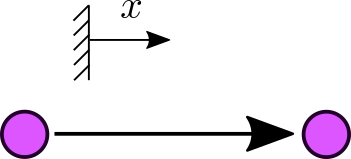
\includegraphics[scale=0.5]{translation.png}
\end{multicols}

\renewcommand{\arraystretch}{1.5}
\begin{tabular}{|l|l} \hline
Position&\hspace{60mm}\\ \hline
Velocity&\\ \hline
Acceleration& \\ \hline
\end{tabular}

}

% Section 2: 
\section{Rotation}

\frame{
\frametitle{Rotation}

\begin{multicols}{2}
Rotational motion is: \vspc
\begin{itemize}
\item motion along a circular path about a fixed point or axis
\item acceleration towards the center of rotation  \vspace{3mm}
\end{itemize}

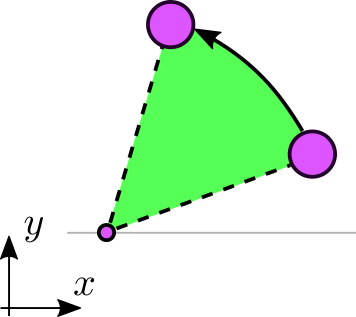
\includegraphics[scale=0.4]{rotation.png}
\end{multicols}

\renewcommand{\arraystretch}{1.5}
\begin{tabular}{|l|l} \hline
Angular Position&\\ \hline
Angular Velocity&\\ \hline
Angular Acceleration&\\
\hline
\end{tabular}

}

\section{Equations of Rotation}

\frame{
\frametitle{Equations of Rotation}

You used these important relationships in your dynamics course. \vspcc

%\scalebox{1}{$\vec{v}=\vec{r}\times\vec{\omega}$} 

With the planar motion assumption this vector equation can be reduced to scalar equation. \vspc

%\scalebox{1}{$v=r\omega$}

}

%Section 3:
\section{Degrees of Freedom}

\frame{
\frametitle{Degrees of Freedom}

The Degrees of Freedom is \vspccc

OR \vspc

The Degrees of Freedom is

}

%Section 4:
\section{DOF Examples}

\frame{
\frametitle{DOF Examples}

Find the degrees of freedom for each of the following systems. \vspcc

\scalebox{.7}{Wittener Metronome \hspace{10mm}Passenger Aircraft \hspace{10mm} Ackermann Steeting Mechanism} \vspc
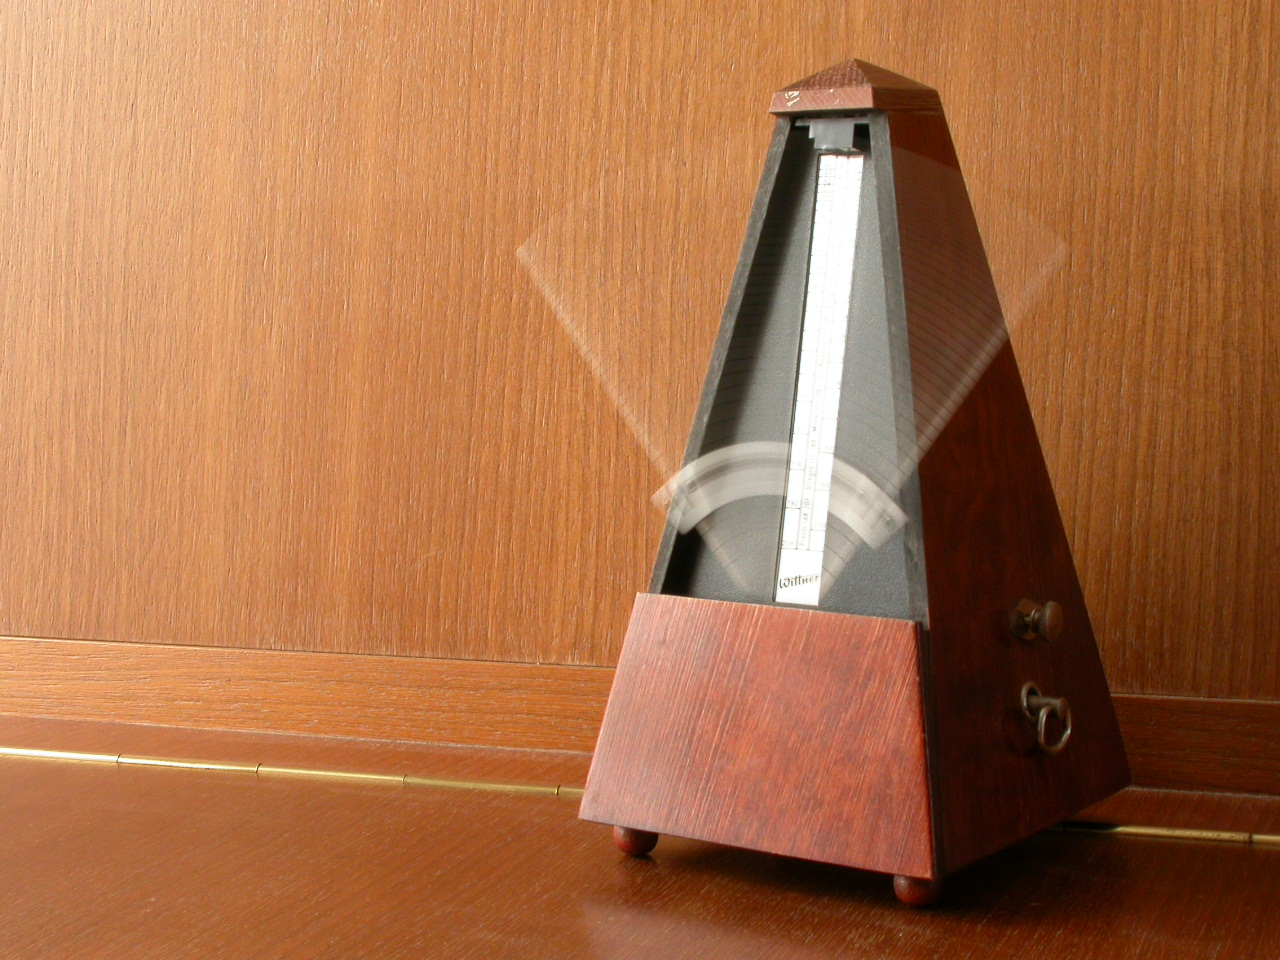
\includegraphics[scale=.25]{Wittner_metronome.jpg} \hspc 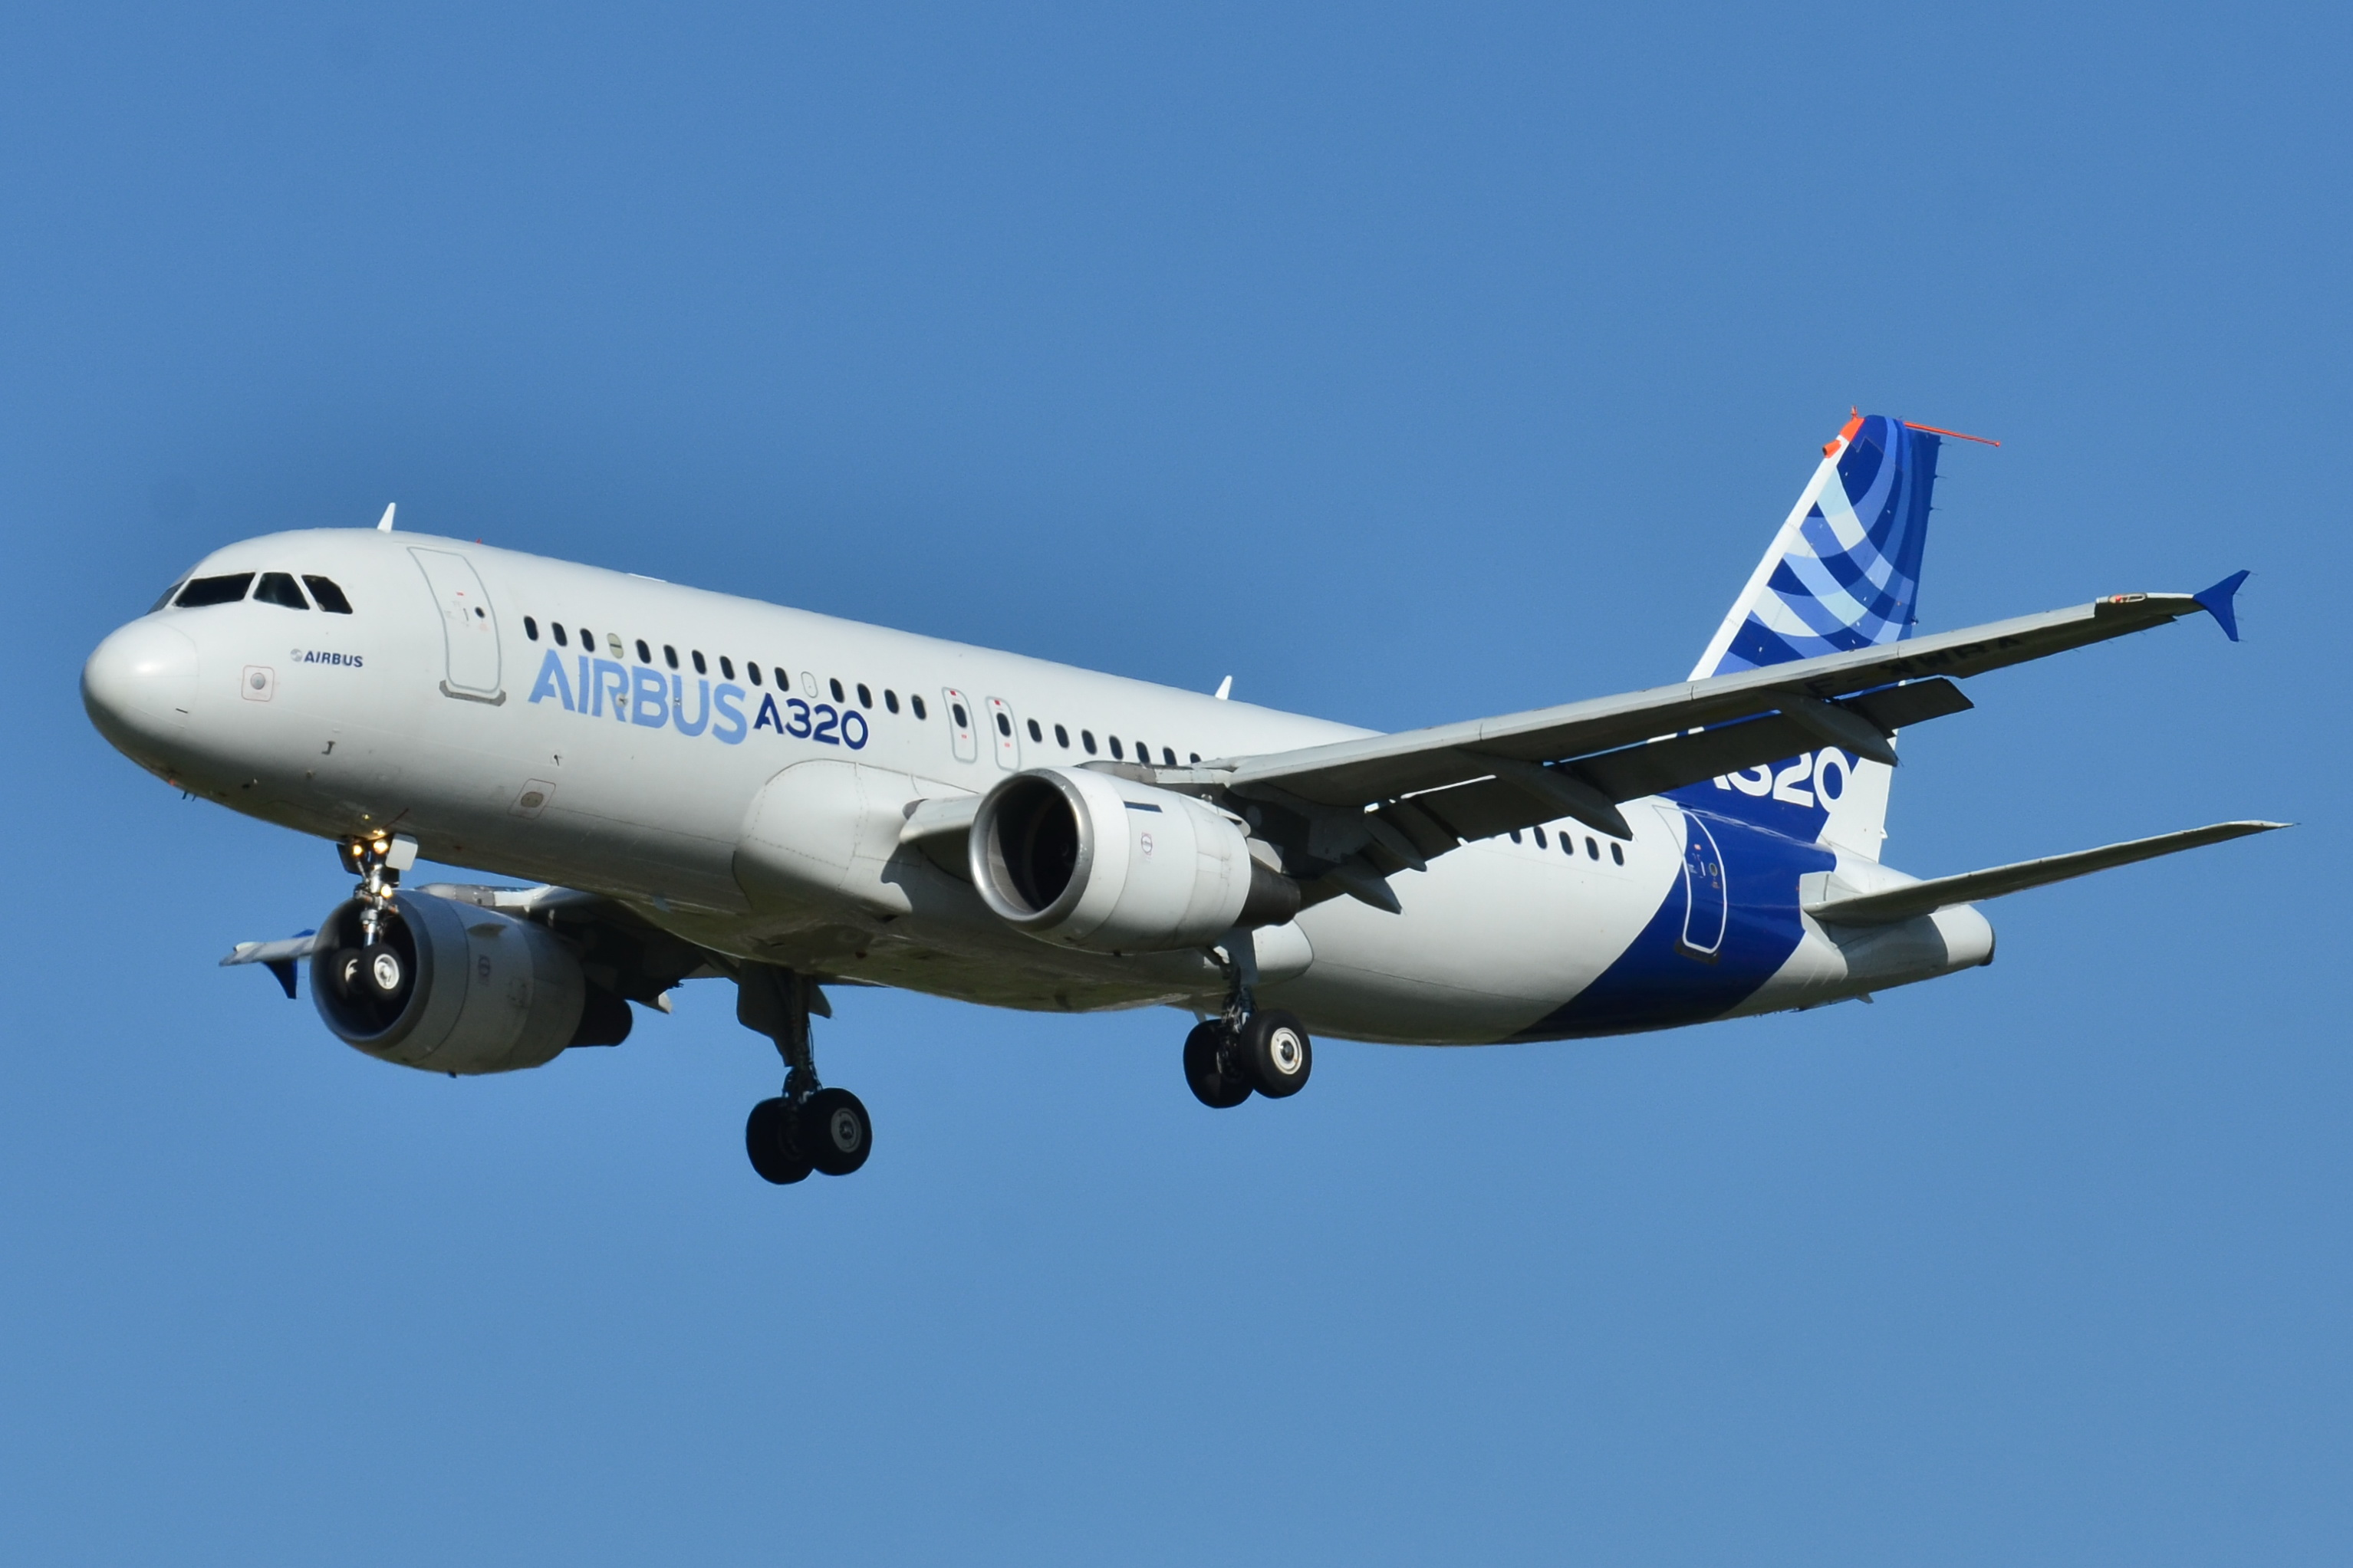
\includegraphics[scale=.125]{airbus_a320.jpg} \hspc 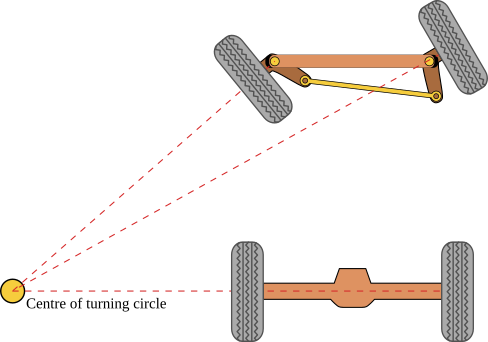
\includegraphics[scale=.25]{Ackermann_turning.png}

{\tiny \href{https://en.wikipedia.org/wiki/Metronome}{Image: Wikipedia}  \hspace{20mm}\href{https://en.wikipedia.org/wiki/Airliner}{Image: Wikipedia} \hspace{20mm}\href{https://en.wikipedia.org/wiki/Ackermann_steering_geometry}{Image: Wikipedia} }
}	
	
\end{document}



